\chapter{Textures}
\label{chap:textures}

\section{Introduction}

The visual world is made of objects (chairs, cars, tables), surfaces (walls, floor, ceiling), and stuff (wood, grass, water). This chapter is about seeing stuff \cite{Adelson2001}. How do we build image representations that can capture what makes wood different from a wall of bricks? 

Representing textures is a task, similar to color perception, that is intimately related to human perception. A texture is a type of image that is composed by a set of similar looking elements. A texture representation contains information about the statistics of its constituent elements, but not about the elements individually. 



In this chapter we will introduce the problems of texture analysis and synthesis as a way to explore texture representations. The models presented here are precursors of more modern approaches using deep learning. But many of the concepts, and some of the intuitions about why these models might be successful, are better understood by exploring first simple yet powerful models. 

Texture synthesis can be solved by a trivial algorithm as shown in \fig{\ref{fig:infinite_texture}}. But such an algorithm, although successful in practice, will give us little understanding on how human perception works and how to modify textures to create new ones. It will also not help us in understanding what representation can be useful to measure similarity between textures. 

\begin{figure}
\centerline{
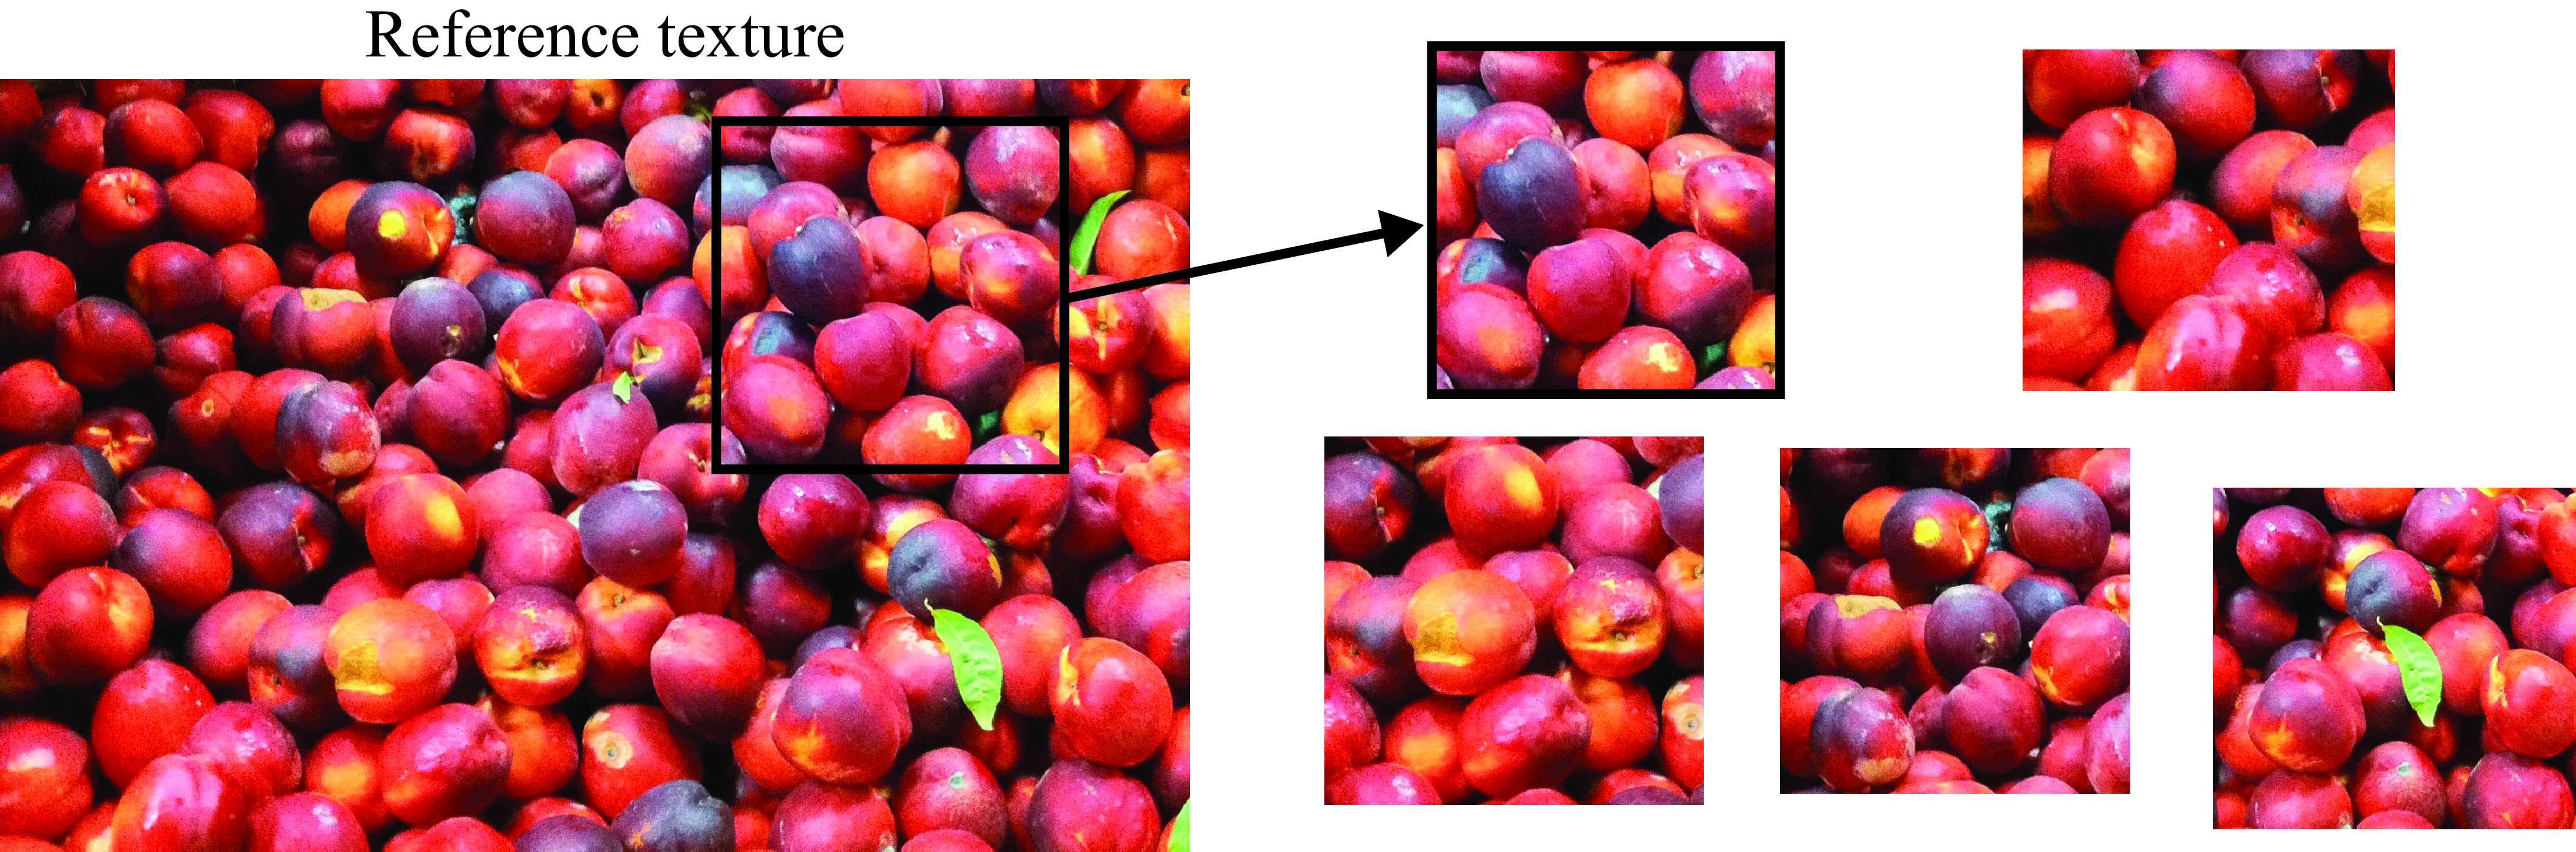
\includegraphics[width=1\linewidth]{figures/heeger_bergen/infinite_texture.eps}
}
\caption{The infinite texture generation algorithm. If we had access to a very large image of the texture we want to generate, we could just crop pieces from it to create new images.  
}
\label{fig:infinite_texture}
\end{figure}


Before we dive into computational approaches to texture analysis, let's first build some intuitions about what might be plausible representations by looking into human perception. 




\section{A Few Notes about Human Perception}


The study of texture perception 
\index{Texture perception}
is a large field in visual psychophysics and we will not try to review it here in detail. Instead, we will just describe three visual phenomena that will allow you getting a sense of the mechanisms underlying texture perception by your own visual system. 

\marginnote{How many stones there are in this wall?
\\[6pt]
\centerline{
\includegraphics[width=.5\linewidth]{figures/heeger_bergen/stone_wall.jpg}}
\\[6pt]
Most people will not care about the number of rocks in the wall, unless you are in the business of selling rocks. Most observers perceive this image as a rock texture.
%Most observers perceive this image as a wall made of many rocks of similar sizes. 
It appears to observers as a texture instead of a composition of countable rocks. They are indeed countable, but counting them requires a significant effort.
}

\subsection{Perception of Sets}

When an image is composed of one or a few distinct objects, we can easily pay attention to each of them individually. We can also count them in parallel, that is, we can tell if an image has one, two, three, or four elements, very quickly and the time it takes for us to say how many elements are in the display does not depend on the number of elements in the image. That is, if a display has only one element or four elements, we are equally fast at reporting that number (figures {\ref{fig:parallel_counting}[a, b and c])}. 


\begin{figure}
\centerline{
\includegraphics[width=1\linewidth]{figures/heeger_bergen/parallel_counting.eps}
}
\caption{When looking at these images, we can count the number of circles at a glance if there are less than five circles. When an image has more than five items, we have to count them one by one. 
}
\label{fig:parallel_counting}
\end{figure}

But something interesting happens when images are composed of more than five similarly looking elements. If we want to count them we need to look at all of them one by one, and the time to count them grows linearly with the number of elements in the image, as illustrated in \fig{\ref{fig:parallel_counting}}. 

The ability to know how many objects are in a display without counting them is called {\bf subitizing}\index{Subitizing} \cite{Kaufman1949}. Subitizing only works when there are fewer than five elements in a display. 

When there are more than four or five objects, we seem to pay attention only to a few of them and represent the rest of them as a set. The perception of sets is an important area of study in human visual psychophysics \cite{Ariely2001}.





\subsection{Crowding}

\Fig{\ref{fig:crowding}} illustrates a curious visual phenomenon.
Look at the central cross and try to read the letter on the left and right without moving your eyes. 

\begin{figure}
\centerline{
\includegraphics[width=1\linewidth]{figures/heeger_bergen/crowding.eps}
}
\caption{Crowding. If you look at the central cross, the letter R on the right can be recognized, however the letter B on the left is hard to read.  
}
\label{fig:crowding}
\end{figure}

You will notice that the letter R on the right can be recognized easily while the letter B on the left is hard to read. The reason cannot be due to the low resolution of peripheral vision as both letters are at the same distance from the fixation location. The explanation of this phenomena is due to something called {\bf crowding}\index{Crowding} \cite{Pell2007}.



As the letter {B is surrounded by other letters, the features of the three letters get entangled as if the pooling window for image features was larger than the three letters together. While you fixate the cross, as you pay attention to the location of the B, you will notice that the features of the three letters are mixed. It is easy to see that it is text, but it is hard to bind the features together to perceive the individual letters. The circles in \fig{\ref{fig:crowding}} represent an approximation of the size of the visual regions over which visual features are pooled. Anything inside the region will suffer from crowding effects. Those regions are larger than what would be predicted by the loss of resolution due to the spacing between receptors in the periphery.

The main message here is for you to feel what it is to perceive what seems to be a statistical representation of the image features present in an image region. 


\subsection{Pre-Attentive Texture Discrimination}

One of the first computational models of texture perception was due to Bela Julesz \cite{Julesz1981}. He proposed that textures are analyzed in terms of statistical relationships between fundamental texture elements that he called {\bf textons}. 
\index{Textons}
It generally required a human to look at the texture in order to decide what those fundamental units were and his models were restricted to binary images formed by simple elements as shown in \fig{\ref{fig:julez_texture}}.


\begin{figure}
\centerline{
\includegraphics[width=.9\linewidth]{figures/heeger_bergen/julez.eps}
}
\caption{Texture discrimination using textons.  
}
\label{fig:julez_texture}
\end{figure}

%Bela Julesz, "Textons, the Elements of Texture Perception, and their Interactions". Nature 290: 91-97. March, 1981. 

One interesting observation about \fig{\ref{fig:julez_texture}} is that it seems easy to see the boundary between the two textures in the image. Interestingly, not all textures can be easily discriminated pre-attentively (i.e., without making an effort). Bela Julesz and many others studied what makes two textures look similar or different in order to understand the nature of the visual representation used by the human visual system.

According to Bela Julesz, textons might be represented by features such as the number of junctions, terminators, corners, and intersections within the patterns. The challenge is that detecting those elements can be unreliable making the representation non-robust.

A different texture representation based on filter banks was introduced in parallel by Bergen and Adelson \cite{Bergen88}, and by Malik and Perona \cite{Malik90}. They showed that filters were capable of explaining several of the {\bf pre-attentive texture discrimination} results, and that features based on filter outputs could be used to do texture-based image segmentation \cite{Malik90}. The texture model we will study in the next section is motivated by those works. 


In the rest of this chapter we will study two texture analysis and synthesis approaches.


\section{Heeger-Bergen Texture Analysis and Synthesis}
\label{section:Heeger_Bergen}
%\subsection{Image synthesis}
The statistical characteristics of image subbands allow for powerful image synthesis and also denoising algorithms. Let's start with the problem of {\bf texture synthesis}\index{Texture synthesis}. The task is as follows: given a reference texture we want to build a process that outputs images with new random samples of the same texture, as shown in \fig{\ref{fig:analysis_heeger_bergen}}. Texture synthesis is important for many computer graphics applications, and also as way of studying what representations of a texture can be useful for visual recognition. 


\begin{figure}
\centerline{
\includegraphics[width=.8\linewidth]{figures/heeger_bergen/analysis_heeger_bergen.eps}
}
\caption{A reference texture image is transformed into a representation using a texture analysis (encoder). Then the texture synthesis procedure takes as input  a random noise image of the size of the desired output texture and the parameters of the reference image $\theta$.
%Texture analysis (encoder) using a steerable pyramid with 4 orientations and 3 scales. The output representation is the concatenation of the 12 subband histograms, the low-pass residual histogram and the input image histogram.  
}
\label{fig:analysis_heeger_bergen}
\end{figure}


%\subsubsection{Heeger-Bergen Texture Synthesis} 


An influential wavelet-based image synthesis algorithm is the Heeger-Bergen texture 
synthesis method published in 1995, with the following origin story \cite{Heeger95Personal}:  David Heeger heard Jim Bergen give a talk at a human vision conference about representations for image texture. 
Bergen highlighted the value of measuring the mean-squared responses of filters applied to images for characterizing texture. He suggested that determining the full probability distribution of each filter's responses would be even more effective. He conjectured that if two textures produced the same distribution of filter responses for all filters, they would look identical to a human observer. Heeger disagreed and aimed to prove Bergen wrong by implementing the proposal using a steerable pyramid \cite{Simoncelli95}.  To Heeger's surprise, the first example he tried worked very well, and this led to Heeger and Bergen's influential paper on texture synthesis \cite{RG:Heeger-Bergen95}.




Texture generation has two stages depicted in \fig{\ref{fig:analysis_heeger_bergen}}. {\bf Texture analysis}\index{Texture analysis} of a reference texture extracts a texture representation, $\theta$. {\bf Texture synthesis} uses a representation, $\theta$, to generate new random samples of the same texture. In the case of texture, it is difficult to precisely define what we mean by ``same texture.'' The perception of textures is an important topic in studies of visual human perception. In general, two textures will be perceived as similar when they seem to be generated by the same physical process.

\marginnote{An important research question is as follows: what is the minimal representation, $\theta$, needed to generate textures that seem identical (i.e., appear as being originated by the same process) to human observers?}

Texture synthesis is usually an iterative image synthesis procedure that begins with a random noise image and uses the parameters $\theta$ to produce a new improved image as shown in \fig{\ref{fig:heeger_bergen_iterations}}. 
We will describe a similar algorithm in \sect{\ref{sec:generative_models:diffusion_models}} when talking about {\bf diffusion models}.

\begin{figure}
\centerline{
\includegraphics[width=1\linewidth]{figures/heeger_bergen/heeger_bergen_iterations.eps}
}
\caption{The steps of the Heeger-Bergen texture synthesis algorithm. The process starts with white noise input image. Each step takes as input the previous output, and it is modified by a function $f_{\theta}$, where $\theta$ are the parameters describing a texture. At each step the output image $x_t$ gets closer to the appearance of the reference texture (\fig{\ref{fig:analysis_heeger_bergen}}). 
%to match the pixel-domain histogram of a source texture image, and then to match, in an image transform domain, the histograms of image subbands of the source texture. The output of that procedure becomes the input to the next iteration.
%A noise input image is modified to match the pixel-domain histogram of a source texture image, and then to match, in an image transform domain, the histograms of image subbands of the source texture. The output of that procedure becomes the input to the next iteration.  
The result of 500 iterations is shown in the right.
}
\label{fig:heeger_bergen_iterations}
\end{figure}



\Fig{\ref{fig:heegersubbands}} shows the main idea behind the approach proposed by Heeger and Bergen to implement the analysis and synthesis functions.  First, the reference texture is decomposed multiple orientation and scales as the outputs of many oriented filters over different spatial scales.  %\fig{\ref{fig:heegersubbands}} shows the multi-scale representation of \cite{Peyre2010}.
The transform should represent all spatial frequencies of the image, so that all aspects of a texture can be synthesized, and the subbands should not be aliased, to avoid artifacts in the synthesized results.
%A steerable pyramid \cite{Simoncelli95} can be used (see \chap{\ref{chapter:image_pyramids}}). 
In the examples shown here we use a steerable pyramid \cite{Simoncelli95} described in \chap{\ref{chapter:image_pyramids}} with six orientations and three scales. The final texture representation is the concatenation of the 18 subband histograms, the low-pass residual histogram and the input image histogram (\fig{\ref{fig:heegersubbands}}[a]). 


\begin{figure}[t]
\centerline{
\includegraphics[width=.8\linewidth]{figures/heeger_bergen/analysis_and_synthesis_heeger_bergen.eps}
}
\caption{(a) Texture analysis (encoder) using a steerable pyramid with six orientations and three scales. The output representation is the concatenation of the 18 subband histograms, the low-pass residual histogram and the input image histogram. (b) Texture synthesis, only one iteration shown. At each iteration, the output is put back as input and the process is repeated $N$ times. The diagram corresponds to the implementation of the function $f_{\theta}$ from \fig{\ref{fig:heeger_bergen_iterations}}.
}
\label{fig:heegersubbands}
\end{figure}

%\begin{figure}
%\centerline{
%\includegraphics[width=1\linewidth]{figures/statistical_image_models/imagestatsA.pdf}
%}
%\caption{The image subbands, and subband filters, for two spatial resolution levels of the source texture image of Fig.~\ref{fig:heegerbergen} (bottom left).
%}
%\label{fig:heegersubbands}
%\end{figure}


 The crux of the algorithm is to alternate matching the intensity domain pixel histogram of the image, then to transform the resulting image into the transform domain and enforce a match, subband by subband, of the image histograms there. 

  \marginnote{Histogram matching is implemented by a pointwise monotonic nonlinearity.}
  
 \Fig{\ref{fig:heegersubbands_histmatch}} shows how one of the subbands gets transformed by the {\bf histogram matching} procedure.\index{Histogram matching} 
 The histogram of the subband of the reference texture has the Laplacian shape typical of natural images. Most of the values of the output of the oriented filter are zero, and only near the triangle boundaries the values are non-zero. In the first iteration, the texture synthesis process starts with white noise (each pixel is sampled independently from a Gaussian distribution). The subband of the input noise has also a Gaussian distribution (as a linear combination of Gaussian random variables also follows a Gaussian distribution). Histogram matching modifies the values of each subband pixel (the histogram matching function is a pixelwise nonlinearity that depends on the current and target pixel histograms). After histogram matching, the noise subband looks sparser, with many values set to zero. The same operation is done for all the subbands in the steerable pyramid. 
 
 
 
 
\begin{figure}[t]
\centerline{
\includegraphics[width=1\linewidth]{figures/heeger_bergen/heeger_bergen_one_subband_tmp.eps}
}
\caption{Histogram matching for one of the subbands. The same operation is done for all the subbands independently.}
\label{fig:heegersubbands_histmatch}
\end{figure}
 
\Fig{\ref{fig:heegersubbands}}{b} shows the result of applying this to all the subbands and then collapsing the pyramid to reconstruct an image. Then we also histogram match the output texture to match the histogram of the pixel values of the reference texture. The result is an image that starts showing some initial black blobs that, after repeating the same process multiple times, will become triangles, as shown in \fig{\ref{fig:heeger_bergen_iterations}}.  After several iterations of the histogram matching steps in both domains (subbands and image) the algorithm appears to converge and the result is the synthesized texture.




The results are often quite good.  For images like the triangles of \fig{\ref{fig:analysis_heeger_bergen}}, the algorithm works well. However, we note that correlations of filter responses across scale is not captured in this procedure, and long or large-scale structures are often depicted poorly. \Fig{\ref{fig:two_examples}} shows two additional examples with more complex images. To process color images, we first do principal component analysis (PCA) in color space to find decorrelated color components, then we apply the texture analysis-synthesis to each decorrelated channel independently. The final image is produced by projecting back into the original color space. For the results in \fig{\ref{fig:two_examples}}, the algorithm is run only for 15 iterations. Adding more iterations makes the images look worse. 


\begin{figure}
\centerline{
\includegraphics[width=1\linewidth]{figures/heeger_bergen/two_examples.eps}
}
\caption{Two examples of synthesized textures. Inputs have a size of 256$\times$256 pixels, outputs are 512$\times$512. In these examples, the algorithm runs for 15 iterations, using a pyramid of six orientation and four scales.}
\label{fig:two_examples}
\end{figure}

 Texture models using statistics of filter outputs are a precursor to diffusion models (\sect{\ref{sec:generative_models:diffusion_models}}) and share a number of architectural features.
 
 The Heeger and Bergen model was one of the first successful approaches that used filter outputs to represent arbitrary textures. Other models followed after that introducing stronger statistical representations capable of generating higher quality textures \cite{Portilla2000}. 

  \marginnote{{\bf Parametric texture models} represent a texture image with a small vector of parameters, usually around 1,000 dimensions \cite{Portilla2000}.}[-.5in]
  
 These models, usually called {\bf parametric texture models}\index{Parametric texture model}, stayed popular until 2000. 
 After that, {\bf nonparametric texture models} became dominant (\sect{\ref{sect:Efros-Leung_texture}}) until generative models with neural networks emerged around 2014. 


%\begin{figure}
%\centerline{
%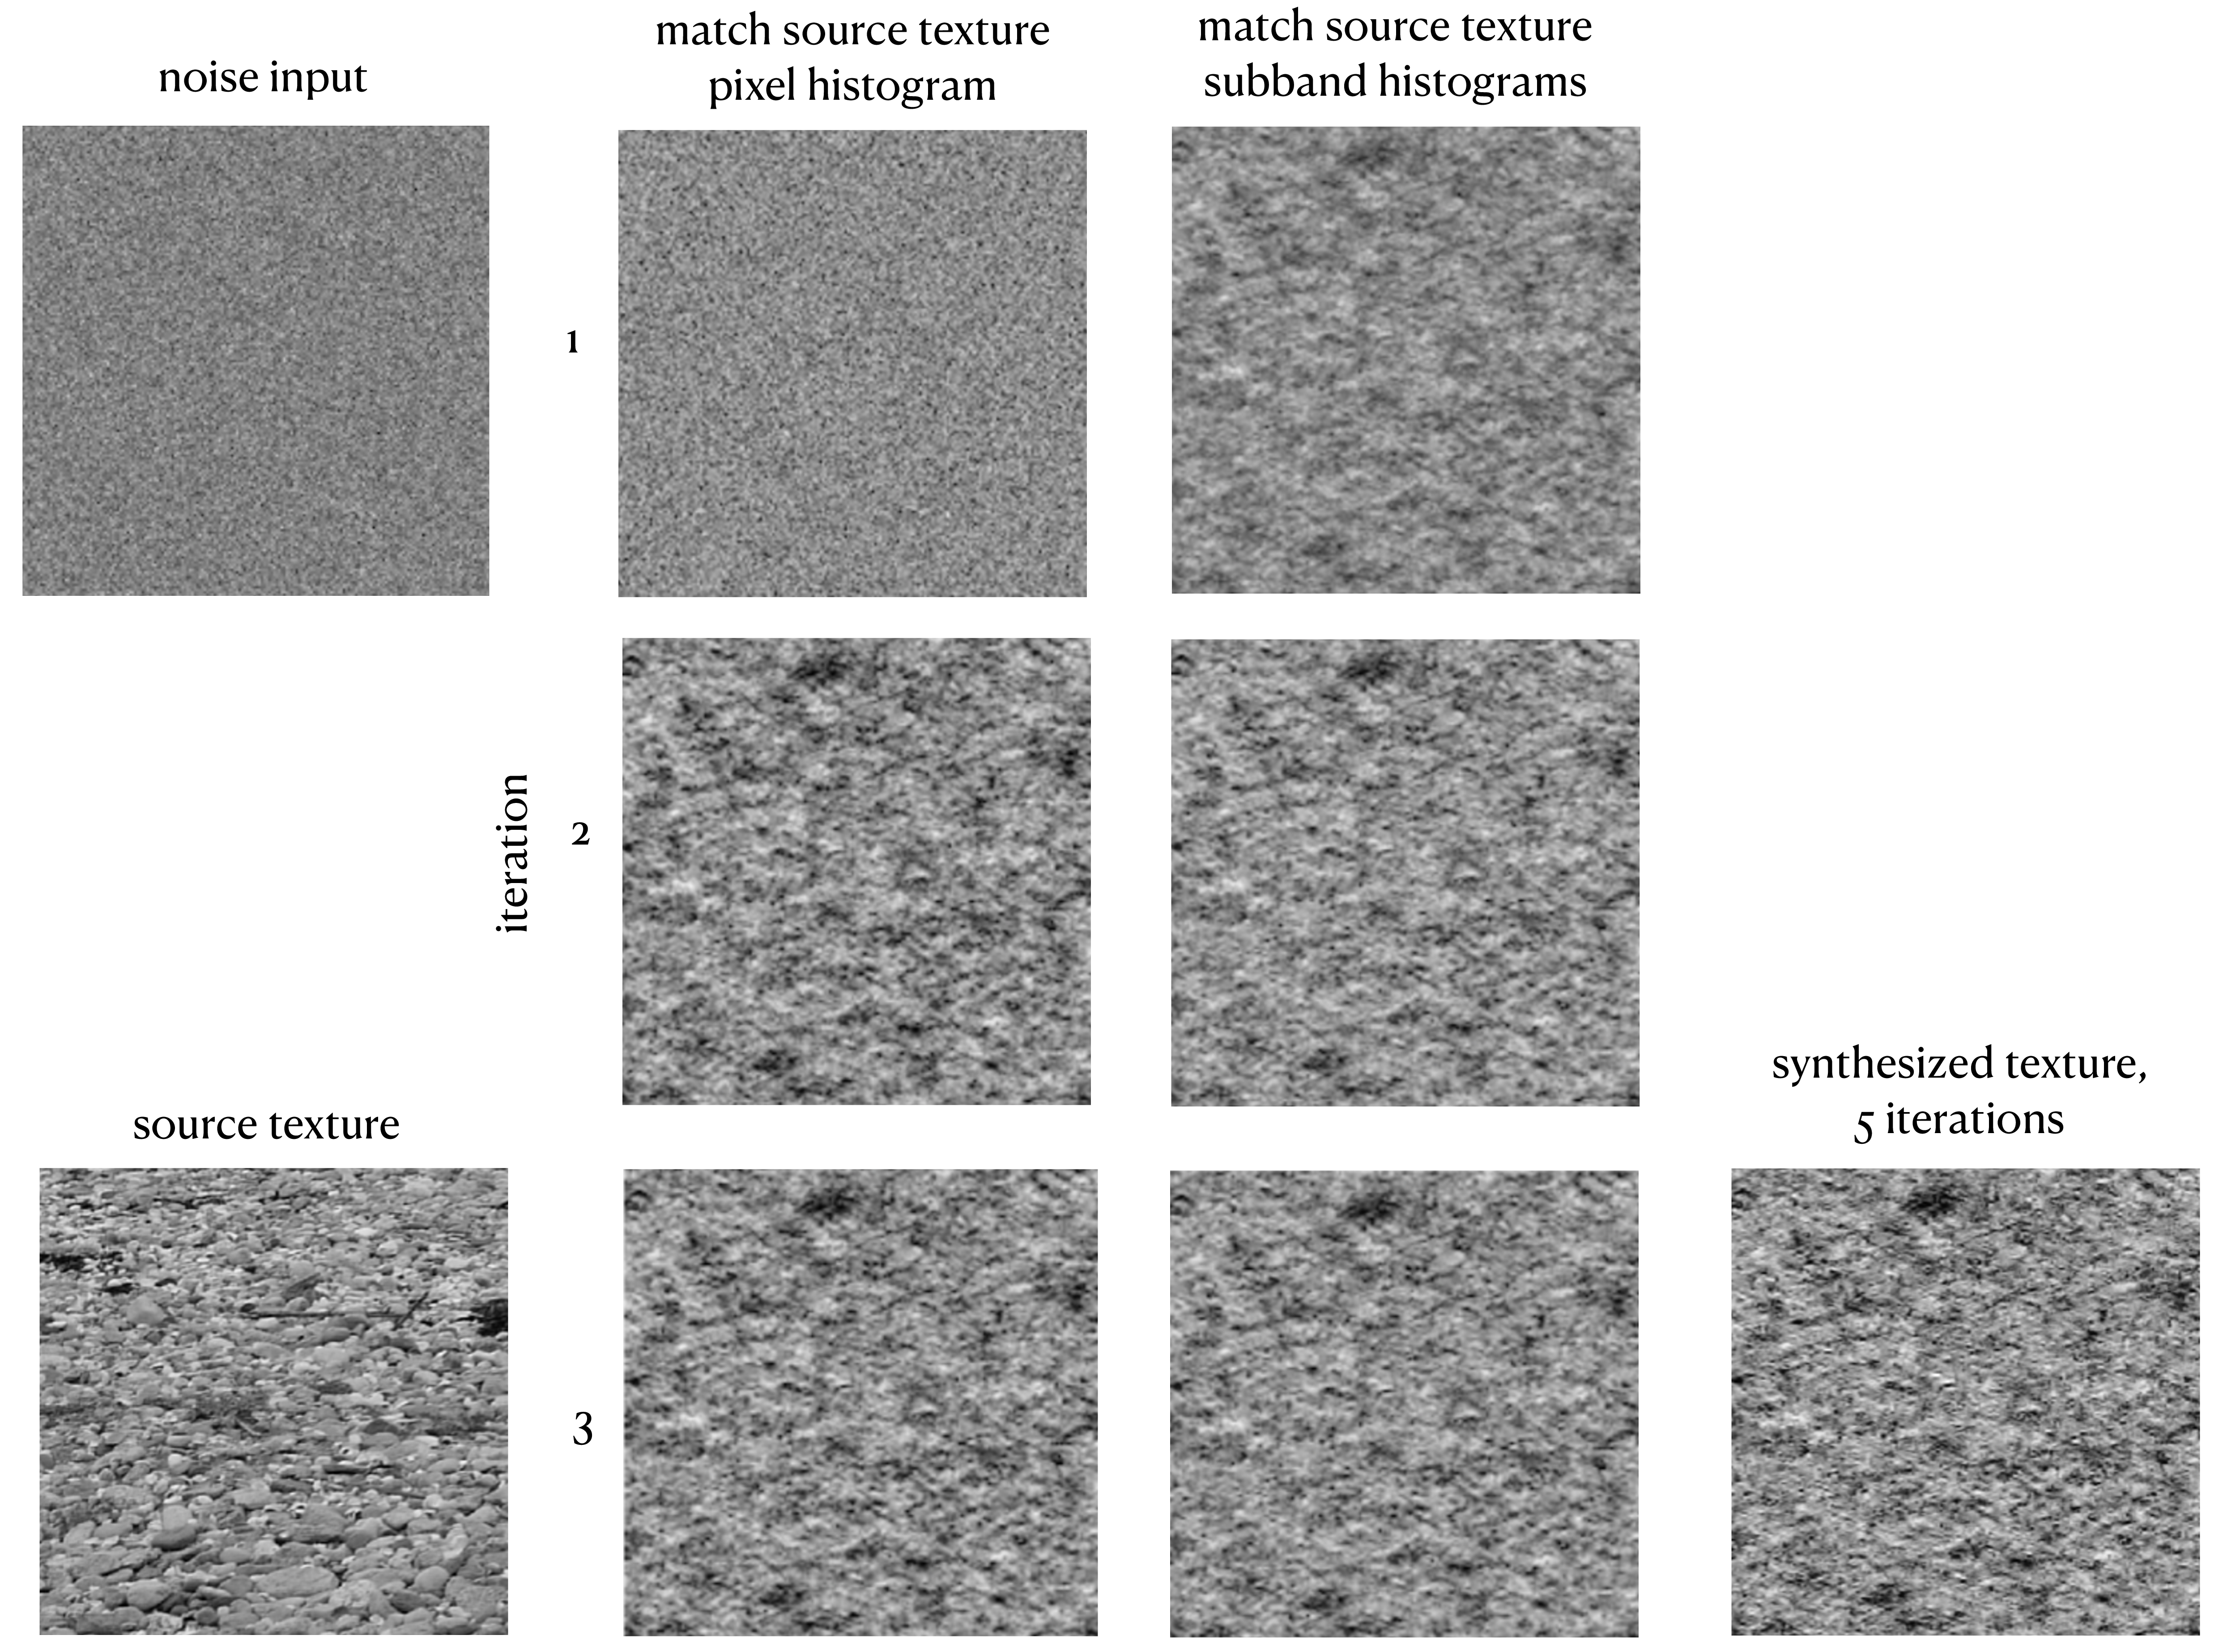
\includegraphics[width=1\linewidth]{figures/statistical_image_models/imagestatsB.pdf}
%}
%\caption{The steps of the Heeger-Bergen texture synthesis algorithm. A noise input image is modified to match the pixel-domain histogram of a source texture image, and then to match, in an image transform domain, the histograms of image subbands of the source texture. The output of that procedure becomes the input to the next iteration.  The result of 5 iterations is shown in the bottom right.
%}
%\label{fig:heegerbergen}
%\end{figure}


\section{Efros-Leung Texture Analysis and Synthesis Model}
\label{sect:Efros-Leung_texture}

Nonparametric Markov random field image models, introduced earlier in \chap{\ref{chapter:stat_image_models}}, define the probability distribution of a pixel as dependent of neighborhood around the pixel. As we said before, if the values of enough pixels surrounding a given pixel are specified, then the probability distribution of the given pixel is independent of the other pixels in the image. This image model can be used as a powerful texture synthesis model \cite{Efros99}.  
\index{Nonparametric texture model}

%A powerful class of image models is known as {\bf Markov Random Field} (MRF) models.  They have a precise mathematical form, which we will describe later, in \chap{\ref{chapter:probabilistic_graphical_models}}.  For now, we present the intuition for these models:  If the values of enough pixels surrounding a given pixel are specified, then the probability distribution of the given pixel is independent of the other pixels in the image.  

As with other texture synthesis algorithms, the input to the Efros-Leung algorithm \cite{Efros99} is an example of the texture to be synthesized, and the output is an image of more of that texture.  It is an iterative algorithm as shown in  \fig{\ref{fig:sampling_efros_leung}}.

\begin{figure}
\centerline{
\includegraphics[width=1\linewidth]{figures/heeger_bergen/sampling_efros_leung.eps}
}
\caption{In the Efros-Leung algorithm \cite{Efros99}, a new pixel in the synthetic texture is created by searching the pixel's neighborhood for similar parts in the reference texture. From $N$ retrieved regions, the central pixels determine the color distribution of the new pixel, generated by randomly selecting one value.
%This illustration shows how a new pixel in the synthetic texture is created in the Efros-Leung algorithm \cite{Efros99}. By using the pixel's neighborhood to search the reference texture for similar parts, $N$ regions are retrieved. The central pixels of these regions represent the color distribution of the new pixel, which is generated by randomly selecting one of those values. %The process continues by repeating the sample process with the following pixel.
%This illustration, shows how a new pixel in the synthetic texture is generated. The neighborhood of the pixel is used to search within the reference texture other similar parts of the image. Once $N$ regions are retrieved, the set of central pixels of the $N$ retrieved patches are used as a representation of the color distribution at that location. The new pixel is generated by taking one of those values at random. 
%Left image shows image texture being synthesized.  The already-synthesized pixels under the green grid define a local context. Regions of the input image which best match that local context are shown at right, and form a set from which to draw a synthesized example.
}
\label{fig:sampling_efros_leung}
\end{figure}

At each iteration, we have synthesized pixels in the neighborhood of the pixel to be synthesized. We look through the input image for examples of similar configurations of pixel values as the current local neighborhood, having a sum of squared intensity differences from the local neighborhood lower than some threshold.  Randomly select one of the matching instances, and copy the value of the pixel into the pixel to be synthesized.  Repeat for all pixels to be synthesized.  It can be natural to synthesize the pixels in a raster-scan ordering.  Image pixels without sufficient neighboring pixels for context can be randomly sampled from the input texture.
\marginnote{In this nonparametric model, the representation of a texture is the reference image itself. There is not a low-dimensional representation as it is the case of parametric texture models. The advantage is that no information is lost in this representation.}[-1.5in]



% Intuitively:  piece of an image is dependent only on the local neighborhood.  In 1-d signals, such a statistical dependence allows for straightforward generation of signals obeying a particular Markov structure, 


% Since images are 2-d structures, it may not be obvious how to generate a 2-d sample obeying a set of conditional statistical relationships.  cite song choon, other mrf.


\Fig{\ref{fig:efros1}} shows how the synthesized texture from the Efros-Leung algorithm \cite{Efros99} changes as a function of size of the context region. \Fig{\ref{fig:efros1}}{a} shows the source texture; \fig{\ref{fig:efros1}}{b} shows how a very small context region (the grid of \fig{\ref{fig:sampling_efros_leung}}) only covers a part of each circle and the synthesized texture doesn't show complete circles; \fig{\ref{fig:efros1}}{c} shows how a larger context region yields a synthesized texture that maintains the circles, but not the regularity of their spacing; and \fig{\ref{fig:efros1}}{d} shows how a still larger context region enforces all the spatial regularities of the input texture.

%\begin{figure}
%\centerline{
%\includegraphics[width=1\linewidth]{figures/statistical_image_models/ELsynth.jpg}
%}
%\caption{Pixel synthesis in the Efros-Leung algorithm \cite{Efros99}.  %Left image shows image texture being synthesized.  The already-synthesized pixels under the green grid define a local context. Regions of the input image which best match that local context are shown at right, and form a set from which to draw a synthesized example.
%}
%\label{fig:efros0}
%\end{figure}

\begin{figure}
\centerline{
\sublabel{a}{\includegraphics[width=0.1\linewidth]{figures/statistical_image_models/efros1a.jpg}}
\sublabel{b}{\includegraphics[width=0.25\linewidth]{figures/statistical_image_models/efros1b.jpg}}
\sublabel{c}{\includegraphics[width=0.25\linewidth]{figures/statistical_image_models/efros1c.jpg}}
\sublabel{d}{\includegraphics[width=0.25\linewidth]{figures/statistical_image_models/efros1d.jpg}}
}
\caption{Synthesized texture from the Efros-Leung algorithm \cite{Efros99} as a function of size of the context region. %(a) The source texture.  (b) A very small context region (the green grid of Fig.~\ref{fig:efros0}) only covers a part of each circle and the synthesized texture doesn't show complete circles.  (c) A larger context region yields a synthesized texture that maintains the circles, but not the regularity of their spacings. (d) A still larger context region enforces all the spatial regularities of the input texture.
}
\label{fig:efros1}
\end{figure}




\Fig{\ref{fig:efrosresult}} shows additional image synthesis results. It is remarkable that such a simple model works so well. The results seem better than the ones shown in \fig{\ref{fig:two_examples}}; however, note that there can still be artifacts (such as the very big leaf that appear in the output). Increasing the neighborhood size can remove those issues. Also, we can see that some elements of the reference texture might appear multiple times in the output texture. Removing repetitions requires decreasing the neighborhood size.


\begin{figure}
\centerline{
\includegraphics[width=1\linewidth]{figures/heeger_bergen/two_examples_efros_leung.eps}
}
\caption{Image synthesis results from the Efros-Leung algorithm.  The small crops are used to synthesize the larger texture regions. Input images are 128$\times$128 pixels, and the outputs are 256$\times$256 pixels. The neighbourhood size is 17$\times$17 pixels. 
}
\label{fig:efrosresult}
\end{figure}

Embellishments have been developed that account for structures over scale \cite{DeBonet98} or which are more efficient by operating on patches \cite{Efros01,Barnes09}. %We will revisit this approach approach when we cover autoregressive models in \chap{\ref{chapter:generative_models}}.


\section{Connection to Deep Generative Models}
In \chaps{\ref{chapter:generative_models}} and \ref{chapter:generative_modeling_and_representation_learning} we will learn about generative models for image synthesis. These chapters cover models that generate images of all kinds, not just textures. However, they have strong similarities to the texture synthesis models we saw in this chapter. A few of connections are as follows:
\begin{itemize}
    \item The Efros-Leung algorithm is an \textbf{autoregressive model}. \Sect{\ref{sec:generative_models:autoregressive}} covers this class of models in more generality, and shows how to use them in conjunction with deep nets.
    \item The iterative optimization of the Heeger-Bergen algorithm is a type of denoising process: it starts with a noise image and little by little transforms it into an image of a texture. This general idea reappears in \sect{\ref{sec:generative_models:diffusion_models}} on \textbf{diffusion models}, which follow this same strategy.
    \item The Heeger-Bergen algorithm is also connected to \textbf{generative adversarial networks} (\textbf{GANs}), which we will encounter in \sect{\ref{sec:generative_models:GANs}}. The objective of Heeger-Bergen is to make a texture that has the same histogram statistics as an exemplar. A GAN also makes images that have the same statistics as a set of exemplars; however, the statistics we seek to match are learned (by a so-called discriminator neural net) rather than hand-defined to be subband statistics.
    \item More generally, texture modeling is about modeling a \textit{distribution over patches}, while generative modeling is about modeling a \textit{distribution over whole images}. The tools are similar in both cases but the scope differs in this way.
\end{itemize}
Be on the lookout for more connections; all generative models are intimately related to each other and it is often possible to frame any one generative model as a special case or extension of any other.

\section{Concluding Remarks}

There is an important relationship between texture models and human perception. One of the goals of many vision algorithms is to compute representations that reproduce image similarities relevant to humans. The representations might be the result of constraining the models to learn human preferences, or as a byproduct of unsupervised learning techniques that result in representations that correlate with human perception. 

The methods described in this chapter are the basis to understand some of the latest image generative models. 
